\section{Firmware}\label{sec:Firmware}
Il firmware per le schede progettate è stato sviluppato utilizzando l'IDE (\textit{Integrated Development Environment}) STM32CubeIDE (versione 1.6.1), una piattaforma di sviluppo C/C++ che permette la configurazione delle periferiche, la generazione e la compilazione del codice e strumenti di debug per i microcontrollori STM32 \cite{STMicroelectronicsSTM32CubeIDE}. \`E basato sul framework Eclipse\textregistered/CDT e sulla toolchain GCC per lo sviluppo e GDB per il debug. Inoltre, si sono utilizzate le librerie HAL (\textit{Hardware Abstraction Layer}), distribuite da STMicroelectronics, che forniscono funzioni e strutture dati utili che agevolano la scrittura del codice. Esse sono state progettate per fornire alcune API (\textit{Application Programming Interface}) per comunicare con i layer superiori delle applicazioni\cite{STMicroelectronicsHAL}. Ogni driver fornito è stato sviluppato seguendo un'interfaccia comune, in modo da standardizzarne la struttura e i nomi di parametri e funzioni. Queste librerie implementano funzionalità utili a gestire le periferiche, in modo da aiutare il programmatore nella scrittura del codice necessario a svolgere alcune attività che tipicamente si usano nei sistemi.
Le principali caratteristiche delle librerie HAL sono:
\begin{itemize}
	\item Insieme di API \textit{cross-family} per l'utilizzo delle periferiche più comuni e API di estensione per particolari funzioni.
	\item Tre modelli di programmazione: polling, interrupt e DMA (\textit{Direct Memory Access}).
	\item Conformità agli standard RTOS (\textit{Real Time Operating System}):
	\begin{itemize}
		\item API completamente rientranti.
		\item Uso sistematico di timeout nella modalità \textit{polling}.
	\end{itemize}
	\item Supporto di istanze multiple di una medesima periferica, permettendo chiamate delle API concorrenti.
	\item Tutte le API implementano un meccanismo di "call-back".
	\item Accesso esclusivo alle risorse condivise.
	\item Utilizzo di timeout per prevenire processi bloccanti.
\end{itemize}

Grazie al \textit{Device Configuration Tool} intregrato nell'ambiente di STM32CubeIDE è possibile generare automaticamente il codice in linguaggio C responsabile dell'inizializzazione della board STM32F4DISCOVERY. In particolare, possono essere configurati tutti i pin e le configurazioni del clock tramite un'interfaccia grafica. La \Fig~\ref{fig:Pinout} mostra la configurazione dei pin utilizzata in questo progetto. 
\begin{figure}[tbh]
	\centering
	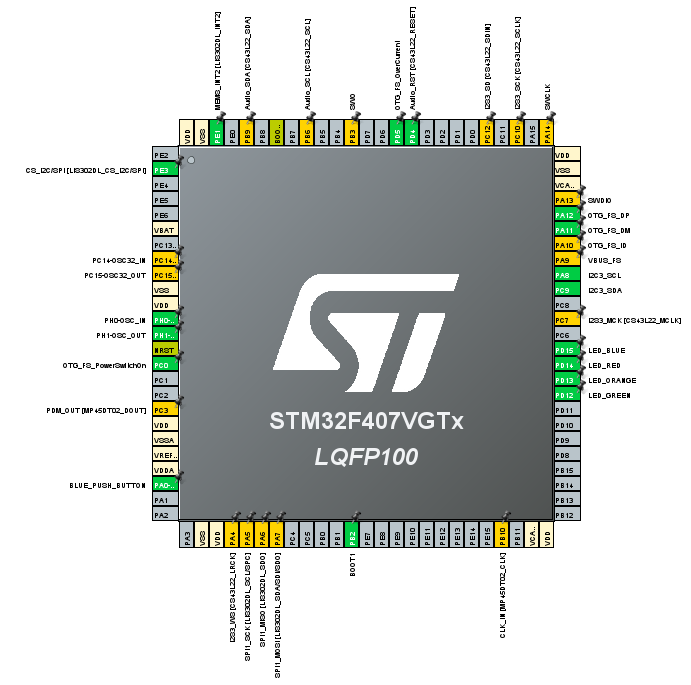
\includegraphics[width=0.9\linewidth]{ImageFiles/Firmware/Pinout}
	\caption{Configurazione pinout della board STM32F4DISCOVERY tramite STM32CubeIDE.}
	\label{fig:Pinout}
\end{figure}
I pin possono essere evidenziati con tre colori:
\begin{itemize}
	\item verde, pin configurato correttamente;
	\item arancio, alcune configurazioni da verificare ma comunque funzionante;
	\item giallo, pin dedicati all'alimentazione;
	\item grigio, pin non utilizzato.
\end{itemize}
Di seguito si riportano le configurazioni dei pin utilizzati per il funzionamento del firmware. Il pin \textit{PA0} è internamente collegato al pulsante \textit{user} già installato sulla board STM32F4DISCOVERY \ref{fig:ImmagineSTM32F4DISCOVERY}. Quando l'utente preme il pulsante viene sollevato un interrupt che verrà catturato dal microcontrollore e permetterà di gestire lo stato del sistema (par. \ref{cap:FSM}). Più precisamente, l'interrupt è sollevato quando viene rilevato un fronte di discesa sul pin associato. Sono stati poi configurati i pin \textit{PD12}, \textit{PD13}, \textit{PD14}, \textit{PD15} che permettono l'accessione e lo spegnimento dei quattro LED integrati sulla scheda. Essi saranno utilizzati per segnalare all'utente lo stato del sistema. Infine, sono stati inizializzati i pin \textit{PA8} e \textit{PC9} per la comunicazione I\ap{2}C con le \textit{Adapter Board}. Infatti, essi svolgono la funzione rispettivamente di linea SCL e SDA.

Il tool permette anche la configurazione del clock della scheda, come mostrato nella figura \ref{fig:Clock}. Per permettere la comunicazione seriale tramite porta USB, si richiede un clock di \SI{48}{\mega\hertz} molto stabile. 
 \begin{figure}[tbh]
 	\centering
 	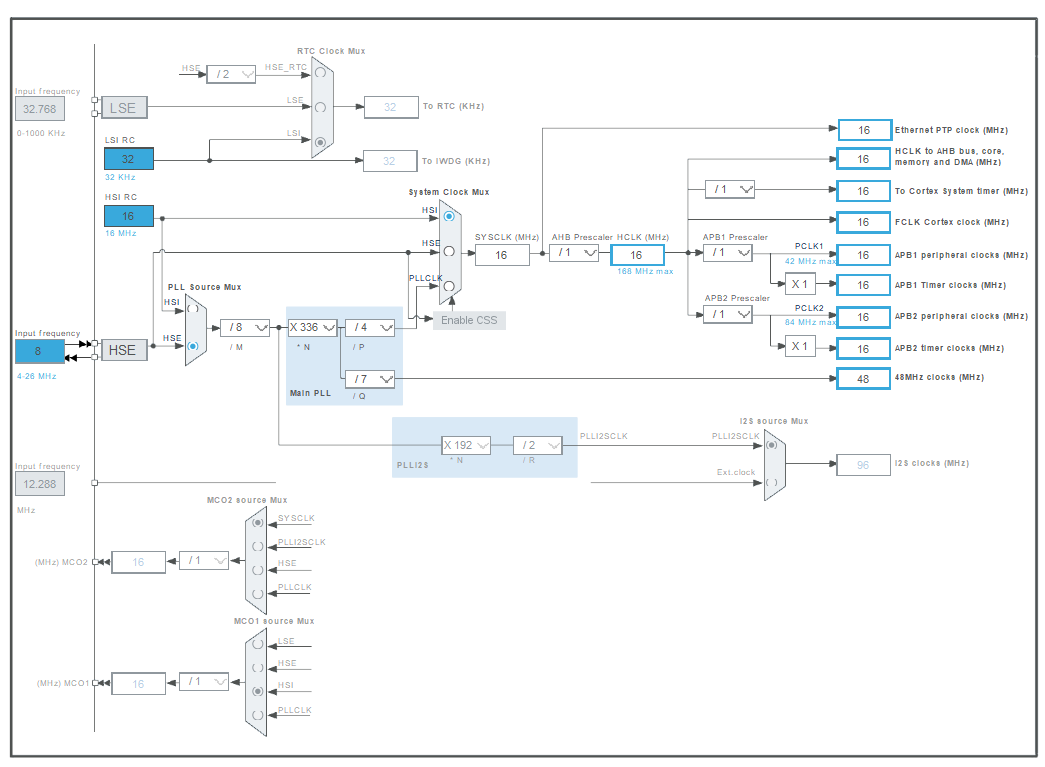
\includegraphics[width=0.9\linewidth]{ImageFiles/Firmware/Clock}
 	\caption{Configurazione clock della board STM32F4DISCOVERY tramite STM32CubeIDE.}
 	\label{fig:Clock}
 \end{figure}
Il clock interno al microcontrollore, abbreviato con la sigla \textit{HSI} (\textit{High Speed Internal}) è tipicamente realizzato con un circuito oscillatorio RC, non molto accurato e può essere influenzato da fattori esterni, come la temperatura. Per questa ragione, si utilizza il segnale proveniente da un cristallo esterno al microcontrollore montato sulla board che fornice una segnale di clock stabile (\textit{HSE}, \textit{High Speed External}). La comunicazione USB è possibile grazie a delle librerie distribuite da STMicroelectronics, che si occupano di inizializzare la comunicazione seriale USB. Inoltre, forniscono il metodo \textit{CDC\_Transmit\_FS}, che permette di inviare un array di tipo \textit{uint\_8} tramite la porta seriale. In questo modo, sarà possibile inviare i campioni acquisiti ad un computer collegato al microcontrollore (vedi par. \ref{cap:FSM}).

\clearpage